(by Vipin Singh)

\p
This chapter presents an analysis of the team structure essential for executing the business model.
It outlines the various roles within the organization and their contributions towards achieving the business objectives.
The focus lies on understanding the division of responsibilities and the collaborative efforts necessary for the company's growth and success.
This examination is intended to provide a clear view of the organizational framework and its significance in the operational realization of the business strategy.

\section{Team composition in the startup phase}
Since the business idea will start in a small scale, the human resources need to be used as efficiently as possible.
With only five founder members, this requires that each members role is not just defined by their job title.
Instead each member will have to be able to adapt and contribute across various facets of the business.
Still the business should also be able to scale up and expand its operations as it grows.

\p
With this said lets analyze the team composition, that is focused to rapidly develop and launch the product.

%TODO: Maybe create the table inline?
\begin{figure}[H]
    \centering
    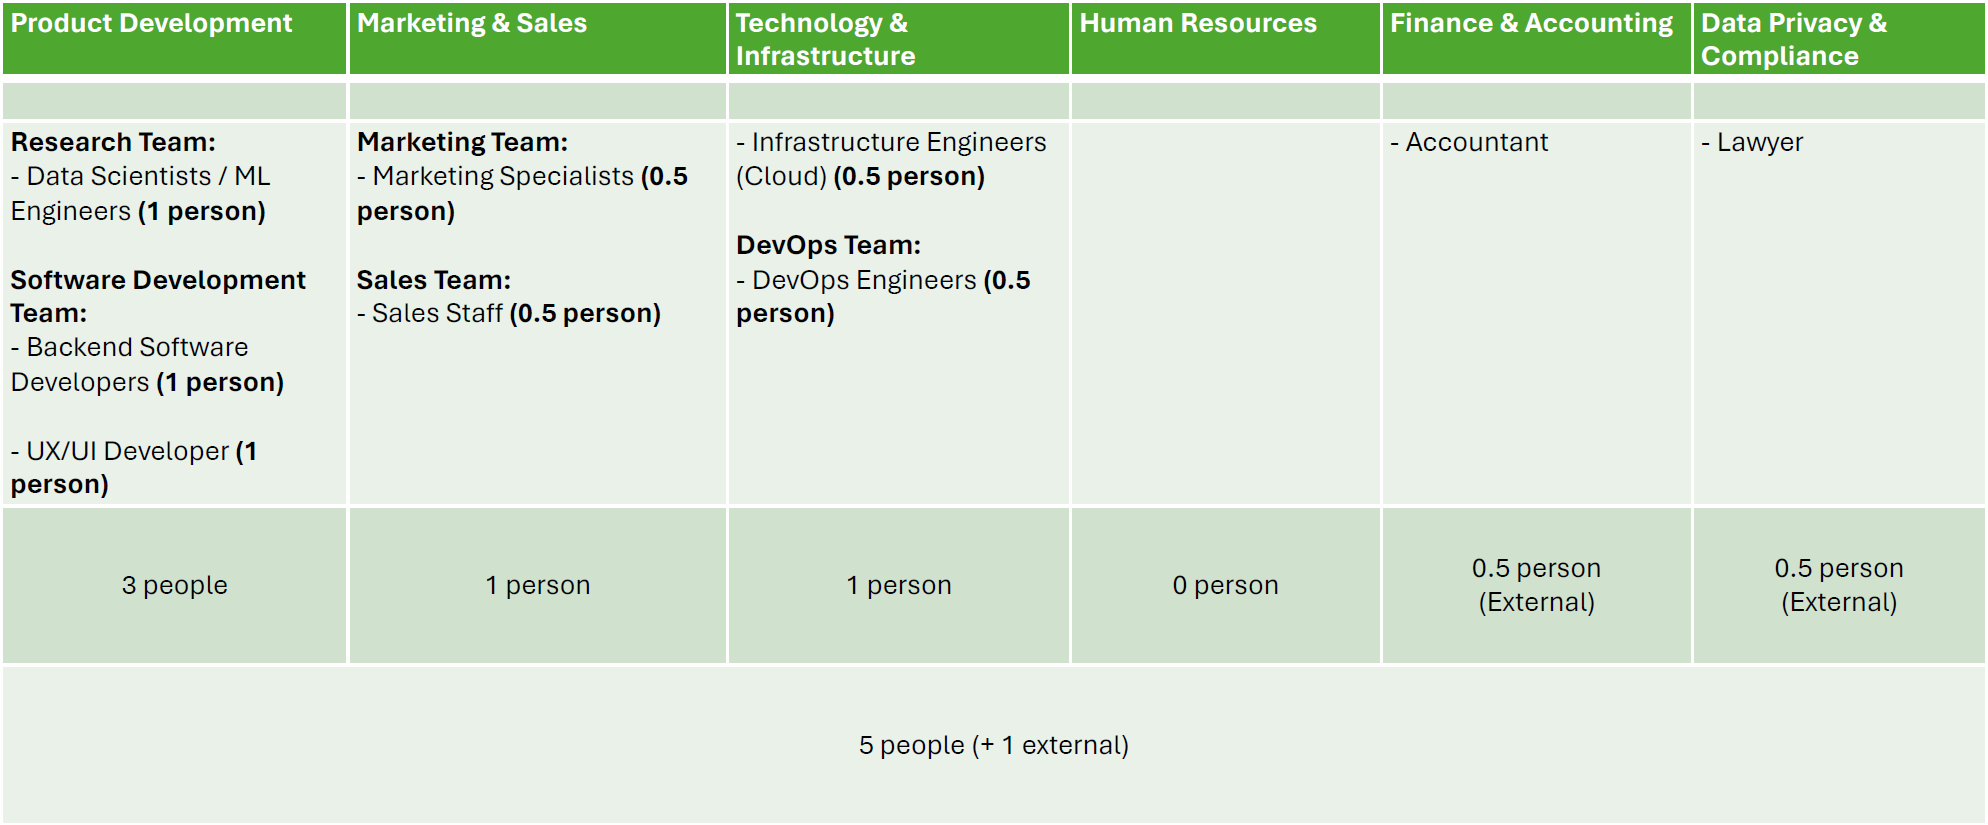
\includegraphics[width=\textwidth]{figures/team_comp_startup.png}
    \caption{Departments with team composition for a startup}
    \label{fig:team_comp_startup}
\end{figure}

In figure \ref{fig:team_comp_startup} we can see the team composition for a startup.
We decided to split the implementation of the team composition into six departments.
This department structure helps us to better understand the responsibilities we must fulfill for the business idea to succeed.
In the following we want to explain the responsibilities of each department and each role within the departments.

\subsection{Product Development}
The product development department is responsible for the development of the product.

\subsubsection*{Research Team}
\begin{itemize}
    \item \textbf{Data Scientists / ML Engineers:} The data scientists and machine learning engineers are responsible for the development of the machine learning models.
\end{itemize}

\subsubsection*{Software Development Team}
\begin{itemize}
    \item \textbf{Backend Software Developers:} The backend software developers are responsible for the development of the backend of the product.
    \item \textbf{UX/UI Developer:} The UX/UI developer is responsible for the development and design of the user interface of the product.
\end{itemize}

\subsection{Marketing \& Sales}
The marketing and sales department is responsible for the marketing and sales of the product.
\subsubsection*{Marketing Team}
\begin{itemize}
    \item \textbf{Marketing Specialists:} The marketing specialists are responsible for the marketing strategy and the marketing team.
\end{itemize}

\subsubsection*{Sales Team}
\begin{itemize}
    \item \textbf{Sales Staff:} The sales staff is responsible for the sales of the product.
\end{itemize}

\subsection{Technology \& Infrastructure}
The technology and infrastructure department is responsible for the technology and infrastructure of the product.
\begin{itemize}
    \item \textbf{IT Support Staff:} The IT support staff is responsible for the IT support of the product.
    \item \textbf{DevOps Engineers:} The DevOps engineers are responsible for the development and operation of the infrastructure of the product.
\end{itemize}

\subsection{Human Resources}
The human resources department is responsible for the human resources of the product.

\subsection{Data Privacy \& Compliance}
The data privacy and compliance department is responsible for the data privacy and compliance of the product.
\begin{itemize}
    \item \textbf{Accountant:} The accountant is responsible for the accounting of the product.
\end{itemize}

\subsection{Finance \& Accounting}
The finance and accounting department is responsible for the finance and accounting of the product.
\begin{itemize}
    \item \textbf{Lawyer:} The lawyer is responsible for the legal aspects of the product.
\end{itemize}

\section{Team composition after higher scaling}
\begin{figure}[H]
    \centering
    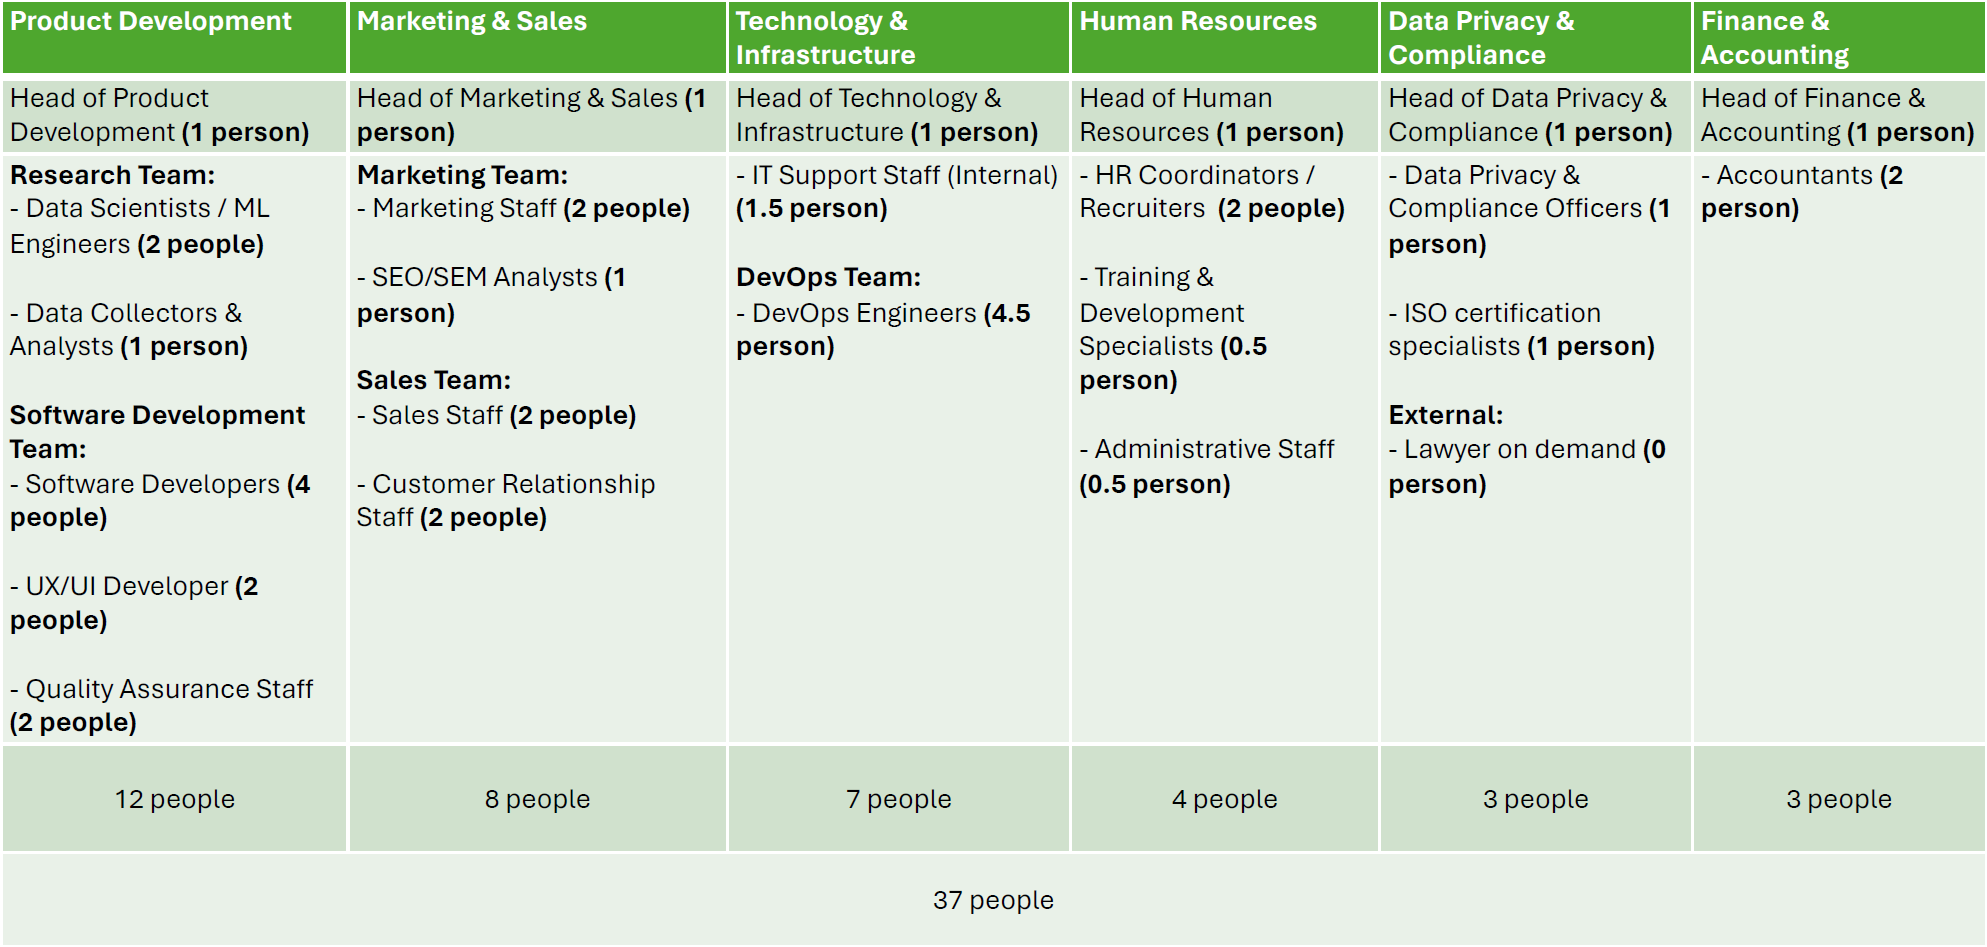
\includegraphics[width=\textwidth]{figures/team_comp_highscaled.png}
    \caption{Departments with team composition after the company has scaled up}
    \label{fig:team_comp_highscaled}
\end{figure}